\chapter{Model dielektrické odezvy DLC vrstev}


KKintegrál, time-reversal symetry a zobecněné f-sum pravidlo.

První podmínka, kterou musí vhodný model lineární dielektrické odezvy splňovat, je Kramers--Kronigův integrál (citovat KK původní články??? nebo nějakou učebnici???), který spojuje reálnou a imaginární část dielektrické funkce  
\begin{equation}
\epsilon_\mathrm{r}(\omega) = 1 + \frac{1}{\pi} \int (preskrtnuty) \frac{\epsilon_\mathrm{i}(\xi)}{\xi - \omega} \mathrm{d}\xi \mathrm{,}
\label{KKint}
\end{equation}
kde $\omega$ je úhlová frekvence a $\epsilon_\mathrm{r}, \epsilon_\mathrm{i}$ jsou reálná a imeginární část dielektrické funkce.  

Druhá podmínka, kterou musí lineární dielektrické odezvy splňovat, je časová symetrie??? (time-reversal symetry)
\begin{equation}
\epsilon(\omega) =\epsilon^* (-\omega) \mathrm{,}
\label{casovasymetrie}
\end{equation}
symbol $^*$ značí komplexní sdružení.

Třetí podmínka, pro model dielektrické odezvy, je takzvané f-sumační pravidlo:
\begin{equation}
\int_0^\infty \epsilon_\mathrm{i} (\omega) \omega \mathrm{d} \omega = \frac{\pi}{2} \omega_\mathrm{p}^2 = \frac{\pi}{2} \frac{e^2 n_\mathrm{e}}{ \epsilon_0 m_\mathrm{e}} \mathrm{,}
\end{equation}
kde $\omega_\mathrm{p}$ je plazmová frekvence, $n_\mathrm{e}$ je koncentrace elektronů, $e$ je elementární náboj a $m_\mathrm{e}$ je hmotnost elektronu. F-sumační pravidlo je důsledek kombinace Kramers-Kronigova integrálu s Newtonovými zákony pro nerelativistickou (klasickou???) nabitou částici a spojuje hustotu náboje s dielektrickou funkcí. Klasické f-sumační pravidlo můžeme chápat jako integrální formu Thomas--Reiche--Kuhnova (TRK) sumačního pravidlo z kvantové mechaniky, pokud ho aplikujeme na intrakci světla s pevnou látkou.  

Klasické sumační pravidlo bylo dále v \cite{sumrule} zobecněno pomocí TKR sumačního pravidla, aby zahrnovalo jak elektrony, tak atomová jádra do následujícího tvaru
\begin{equation}
\int_0^\infty "F" \mathrm{d}E = n_e + \sum_n \frac{Z_n^2 m_\mathrm{e}} {m_\mathrm{n}} n_\mathrm{n} = U n_\mathrm{e} \mathrm{.} %FIXME
\end{equation}
Sumace je prováděna přes všechny typy jader v materiálu. Symboly $Z_\mathrm{n}, m_\mathrm{n}, n_\mathrm{n}$ značí pořadě protonové číslo, hmotnost jádra a koncentraci jader. Faktoru $U$ je pro většinu materiálů velmi podobný: $U = 1.00027$ \ref{sumrule???}.

Funkci $"F"(E)$ nazýváme funkce síly přechodu. Pro parametrizaci dielektrické funkce je praktické zavést funkci
\begin{equation}
F(E) = \epsilon_\mathrm{i}(E) E = \frac{"F(E)"}{M}\mathrm{,}
\end{equation}  
kde $M$ je konstanta:
\begin{equation} 
M = \frac{8 \pi \epsilon_0 m_\mathrm{e}}{(e h)^2} = 4,61706\times10^{26} \mathrm{eV}^{-2}\mathrm{m}^3 \mathrm{.}
\end{equation}

Funkci $F(E)$ můžeme také nazývat funkce síly přechodu a slouží jako výchozí bod při parametrizaci optických konstant v pevných látkých.

\section{Parametrizace funkce dielektrické odezvy}
Dielektrická funkce je seskládána z jednotlivých částí, které reprezentují jednotlivé typy přechodů $t$. Celková dielektrická funkce je suma přes dielektrické funkce jednotlivých částí a vakua \cite{sumrule1}. 
\begin{equation}
\epsilon(E) = 1 + \sum_t \epsilon_t(E)
\label{suma1}
\end{equation}

Dále zavedem takzvanou "funkci síly přechodu (transition strength function)"? $F(E)$ která se skládá z funkci síly přechodu pro jednotlivé říspěvky t.
\begin{equation}
F(E) = \sum_t F_t(E)
\end{equation}
Je praktické jednotlivé příspěvky $F_t$ normalizovat na $F_t^0$ aby platilo
\begin{equation}
\int_0^\infty F_t^0(E)\mathrm{d}E = 1
\end{equation}

Integrováním přes $F_t(E)$ získáme 
\begin{equation}
\label{definiceceelkovesily}
\sum_t \int_0^\infty F_t(E)\mathrm{d}E = \sum_t N_t = N \mathrm{.}
\end{equation}
$N_t$ jsou integrální síly přechodů pro jednotlivé příspěvky a $N$ je celková integrální síla přechodu, nebo jen jednoduše celková síla přechodu.  

Podobně můžeme zavést takzvanou normalizovanou dielektrickou funkci $\epsilon_t^0$ pro jednotlivé příspěvky. Platí 
\begin{equation}
\epsilon_t(E) = N_t \epsilon_t^0  \, \mathrm{,}
\end{equation}
kde $N_t$ je takzvaná integrální síla přechodu pro jednotlivé příspěvky.

Pak můžeme přepsat rovnici (\ref{suma1}) jako:
\begin{equation}
\epsilon (E) = 1 + \sum_t N_t \epsilon_t^0(E) \mathrm{.}
\end{equation}




\section{Jednotlivé přespěvky k dielektrické funkci}
Jelikož se v této práci zabýváme zkoumáním DLC vstev deponovaných na krystalickém křemíku, 




\subsection{Mezipásové přechody mezi valenčním a vodivostním pásem}
%FIXME: použijeme tohle vůbec??? V amorfním materiálu s jedním valenčním a vodivostním pásem je příspěvek k dielektrické funkci nenulový v intervalu energií od $E_\mathrm{g}$ do $E_\mathrm{h}$, kde $E_\mathrm{g}$ je šířka zakázaného pásu a $E_\mathrm{h}$ je rozdíl energií mezi minimem valenčního a maximem vodivostního pásu (maximální energie přechodu mezi valenčním a vodivostním pásem). Následující parametrizace se ukázala jak vhodná. FIXME!

Absorpce světla v amorfních nebo krystalických materiálech je způsobena přechodem elektronu z výchzího stavu $j$ s energií $S$ do konečného stavu $k$ s energií $S + E$. Imaginární část dielektrické funkce je spočítána jako suma příspěvků všech možných přechodů:

\begin{equation}
\label{basicDOS}
\epsilon_\mathrm{i} (E) = 
\left(\frac{eh}{m_\mathrm{e}E} \right)^2 \frac{1}{4 \pi \epsilon_0 \mathrm{B}_0} \sum_{j,k} | p_{j \rightarrow k} |^2
\int_{-\infty}^\infty f_\mathrm{e}(S) \mathcal{N}_j(S) f_\mathrm{h}(S+E) \mathcal{N}_k(S + E)\mathrm{d}S \text{,}
\end{equation}
kde $E$, $h$, $\epsilon_0$ a $\mathrm{B}_0$ jsou energie fotonu, Planckova konstanta, permitivita vakua a příslušná část Brillouinovy zóny odpovídajícího krystalického materiálu. Funkce $\mathcal{N}_j(S)$ a $\mathcal{N}_k(S)$ značí rozdělení energií hustoty stavů (DOS) v $j$ a $k$ pásu. Koncentrace $j$ elektronů, tj. počet $j$ elektronů na jednotku objemu je definován takto:
\begin{equation}
\mathrm{N}_j = \int_{-\infty}^\infty \mathcal{N}_j(S)\mathrm{d}S \text{.}
\end{equation}
Výše uvedené přechody jsou možné pouze, pokud je jsou $j$ stavy zaplněné and $k$ stavy nejsou. Toto můžeme zahrnout přidáním Fermi-Diracova rozdělení pro elektrony, $f_\mathrm{e}$, a díry, $f_\mathrm{h}$, do integrálu. Pravděpodobnost přechodu je dána čtvercem prvku matice hybnosti (squared momentum-matrix element???) $|p_{j \rightarrow k}|^2$. Je vytknuta před integrál, protože předpokládáme, že je konstantní pro všechny přechody mezi konkrétním $j$ a $k$ pásem. Rovnice (\ref{basicDOS}) může zahrnovat jednak mezipásové přechody i přechody v do vyšších stavů v rámci pásu (intraband transitions????). DOS funkce ${N}_j(S)$ a $\mathcal{N}_k(S)$ můžou také zahrnovat jedna rozšířené a jednak lokalizované stavy. Pokud je nicméně valenční pás plně zaplněn a vodivostní pás je zcela prázdný, můžeme Fermi-Diracovo rozdělení vynechat a inergál v rovnici (\ref{basicDOS}) poté definuje tzv. funkci sdružené hustoty stavů (JDOS) $\mathcal{J}_{j \rightarrow k}(E)$ odpovídající $j \rightarrow k$ přechodům
\begin{equation}
\mathcal{J}_{j \rightarrow k}(E) = \int_{-\infty}^\infty \mathcal{N}_j(S) \mathcal{N}_k(S + E)\mathrm{d}S \text{.}
\end{equation}
Rovnice (\ref{basicDOS}) nicméně definuje pouze imaginární část dielektrické funkce a pouze pro kladné $E$. Celkovou komplexní dielektrickou funkci můžeme získat pomocí antisymetrie imaginární části (\ref{casovasymetrie}) a Kramers-Kronigových relací (\ref{KKint}):
\begin{equation}
\epsilon_i (E) = 
\left(\frac{eh}{m_\mathrm{e}E} \right)^2 \frac{\mathrm{sgn}{E}}{4 \pi \epsilon_0 \mathrm{B}_0} \sum_{j,k} | p_{j \rightarrow k} |^2
\int_{-\infty}^\infty f_\mathrm{e}(S) \mathcal{N}_j(S) f_\mathrm{h}(S+E) \mathcal{N}_k(S + E)\mathrm{d}S \text{,}
\end{equation}

\begin{equation}
\epsilon_\mathrm{r}(E) = 
1 + \frac{1}{\pi} \mathcal{P} \int_{-\infty}^\infty \frac{\xi \epsilon_\mathrm{i}(\xi)}{\xi^2 - E^2} \mathrm{d}\xi = 
1 + \frac{2}{\pi} \mathcal{P} \int_0^\infty \frac{\xi \epsilon_\mathrm{i}(\xi)}{\xi^2 - E^2} \mathrm{d}\xi 
\text{.}
\end{equation}


Vhodný model proto můžeme sestrojit buď parametrizací DOS funkcí, příklad takového modelu publikoval Dan Franta \ref{franta20007}. Nevýhodou paramatrizace     

V \ref{} je model PJDOS rozšířen dále o parametry $E_\mathrm{c}$ a $B_\mathrm{c}$ zahrnující rozšíření pásové struktury a její nesymetrii vzhledem k Fermiho energii?????

\begin{equation}
\label{valencvod}
\epsilon_\mathrm{i,vc}^0 = \mathrm{sgn}(E) \frac{(|E|- E_\mathrm{g})^2(E_\mathrm{h} - |E|)^2}{ C E^2 [(|E| - E_\mathrm{c})^2 + B_\mathrm{c}^2]} \Pi_{E_\mathrm{g},E_\mathrm{h}}(|E|) \, \mathrm{,}
\end{equation}
kde 

Funkce $\Pi_{E_\mathrm{min},E_\mathrm{max}}(|E|)$ je definována následovně:
\begin{equation}
\Pi_{E_\mathrm{min},E_\mathrm{max}}(|E|) = 
	\left\{\begin{array}{l l} 
	1 : E_\mathrm{min} < E < E_\mathrm{max} \\
	0 : \text{jinak.} \end{array} \right.
\end{equation}

\subsection{Excitace elektronů do vyšších vodivostních pásů}
\begin{equation}
a
\end{equation}


\subsection{Fononová absorpce}
V infračervené oblasti se v DLC vrstvách výskytuje velké množství absorpčních píků, způsobených absorpcí na vibračních stavech C a C--H skupin. Jednotlivé píky je možno modelovat jako Gausovské píky v imaginární části dielektrické funkce \cite{franta2007}:

\begin{equation}
\epsilon^0_{\mathrm{i},p} = \frac{1}{\sqrt{2 \pi} B_p E_p} \left[ \exp\left(-\frac{(E-E_p)^2}{2B_p^2}\right) - \exp\left(-\frac{(E+E_p)^2}{2B_p^2}\right) \right] \text{.}
\end{equation}
V reálné části tomu odpovídá tvar:
\begin{equation}
\epsilon^0_{\mathrm{r},p} = \frac{-\sqrt{2}}{\pi B_p E_p} \left[ \mathrm{D}\left(\frac{E-E_p}{\sqrt{2}B_p}\right) - \mathrm{D}\left(\frac{E+E_p}{\sqrt{2}B_p}\right) \right] \text{,}
\end{equation}
kde $\mathrm{D}(x)$ značí Dawsonův integrál, definovaný jako:
\begin{equation}
\mathrm{D}(x) = \exp(-x^2)\int_0^x \exp(t^2) \mathrm{d}t
\end{equation}
V infračervené spektroskopii je nicméně zvykem používat k popisování píků vlnočty místo energií. Z toho důvodu jsou parametry $E_p$ a $B_p$ nahrazeny parametry $\nu_p$ a $\beta_p$:
\begin{equation}
E_p = h c \nu_p \text{,}
\end{equation}
\begin{equation}
B_p = \frac{h c \beta_p}{2 \sqrt{2 \ln 2}} \text{,}
\end{equation}
kde $h$ je Planckova konstanta a $c$ je rychlost světla. 


\subsection{Excitace jaderných elektronů}



\section{Aplikace na DLC vrstvy (model PJDOS-DLC)}
V této práci byly DLC vzorky modelovány jako multivrstva: systém vrstva -- přechodová vrstva -- substrát -- zadní vrstva (obrázek \ref{}). Pro modelování dielektrické funkce vrstvy byl použit model PJDOS-DLC, pro modelování přechodové vrstvy byl použit model PJDOS, 

\subsection{Vrstva}
Pro modelování dielektrické funkce DLC vrstvy byl použit model PJDOS-DLC \cite{franta2007}. Ten zahrnuje jednak přechody mezi valenčním a vodivostním pásem (\ref{valencvod}) pro $\sigma$ a $\pi$ elektrony, pak také excitace do vyšších excitovaných stavů nad vodivostním pásem \ref{}, absorpci na vibračních stavech v infračervené oblasti \ref{gaus} a excitaci jaderných elektronů \ref{jaderneel}. Zjednodušené schéma elektronové struktury DLC vrstvy je na obrázku \ref{DLCDOS}.

\begin{figure}[h]
\centering
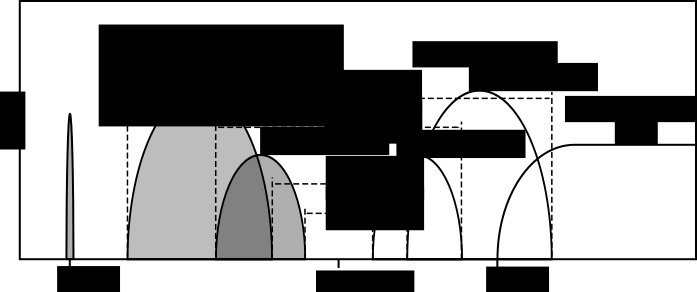
\includegraphics[width=15cm]{grafika/DLCDOS.pdf}
\caption{DOS}
\label{DLCDOS}
\end{figure} 

DLC vrstvu uvažujeme jako systém tří komponent: vodíkových jader, uhlíkových jader a elektronů. Celkovou sílu přechodu $N$ můžeme proto rozepsat jako:
\begin{equation}
N = \int_0^\infty \epsilon_\mathrm{i}(E) E \mathrm{d}E = N_\mathrm{e} + N_\mathrm{C} + N_\mathrm{H} \text{,}
\end{equation} 
kde $N_\mathrm{e}$, $N_\mathrm{C}$ a $N_\mathrm{H}$ jsou částečné síly přechodu pro elektrony, uhlíková jádra a vodíková jádra. Pro uhlíky můžeme navíc rozlišit sílu přechodu pro sp2 a spc3 vázaný uhlík $N_\mathrm{C_{sp3}}$, $N_\mathrm{C_{sp2}}$
\begin{equation}
N_\mathrm{C} = N_\mathrm{C_{sp3}} + N_\mathrm{C_{sp2}} \text{.}
\end{equation} 
Jednotlivé síly přechodů závisí pouze na složení a hustotě systému:
\begin{equation}
N_\mathrm{e} = [Z_\mathrm{C}(f_\mathrm{C}) + Z_\mathrm{H} f_\mathrm{H}] N_\mathrm{a} = (6f_\mathrm{C} + f_\mathrm{H})N_\mathrm{a} \text{,}
\end{equation}
\begin{equation}
N_\mathrm{C} = Z^2_\mathrm{C} f_\mathrm{C} \frac{m_\mathrm{e}}{m_\mathrm{C}} N_\mathrm{a} = const f_\mathrm{C} N_\mathrm{a} \text{,}
\end{equation}
\begin{equation}
N_\mathrm{H} = Z^2_\mathrm{H} f_\mathrm{H} \frac{m_\mathrm{e}}{m_\mathrm{H}} N_\mathrm{a} = 0,000545 f_\mathrm{H} N_\mathrm{a} \text{,}
\end{equation}
kde $N_\mathrm{a}$ značí atomovou koncentraci a $f_\mathrm{H}$, $f_\mathrm{C}$ jsou koncentrace vodíku a uhlíku ($f_\mathrm{H} + f_\mathrm{C} = 1 $). $Z_\mathrm{C}$ a $Z_\mathrm{H}$ značí atomové čísla uhlíku a vodíku. $m_\mathrm{e}$, $m_\mathrm{C}$ a $m_\mathrm{H}$ jsou hmotnost elektronu, hmotnost jádra uhlíku a hmotnost jádra vodíku. 

Celkovou sílu přechodu $N$ také můžeme vyjádřit podle (\ref{definiceceelkovesily}) jako součet jednotlivých příspěvků $t$

\begin{equation}
N = N_\mathrm{v} + N_\mathrm{K} + N_\mathrm{f} \text{.}
\end{equation}

$N_\mathrm{v}$ zde značí sílu kombinovanou sílu přechodu pro valenční elektrony jednak do vodivostního pásu a jednak do excitovaných stavů nad vodivostním pásem. $N_\mathrm{v}$ můžeme rozložit na části pro $\sigma$ a $\pi$ elektrony $N_\sigma$, $N_\pi$ podle jejich poměru (na jeden sp2 atom uhlíku připadá jeden $\pi$ elektron a tři $\sigma$ elektrony, na sp3 vázaný uhlík čtyři $\sigma$ elektrony a na vodík pouze jeden $\sigma$  elektron)
\begin{equation}
N_\sigma = N_\mathrm{v} \frac{f_\mathrm{C_{sp2}}}{4f_\mathrm{C} + f_\mathrm{H}}  \text{,}
\end{equation}
\begin{equation}
N_\pi = N_\mathrm{v} \frac{4f_\mathrm{C_{sp3}} + 3f_\mathrm{C_{sp2}} + f_\mathrm{H}}{4f_\mathrm{C} + f_\mathrm{H}}  \text{.}
\end{equation}

$N_\sigma$ a $N_\pi$ můžeme opět rozložit na části určující sílu přechodů mezi valenčním a vodivostním pásem a mezi valenčním pásem a vyššími excitovanými stavy
\begin{equation}
\begin{array}{lr}
N_{\sigma \rightarrow \xi} = N_\mathrm{\sigma} \alpha_{\sigma\xi} \text{,} &
N_{\sigma \rightarrow \sigma^*} = N_{\sigma \rightarrow \xi} - N_{\sigma \rightarrow \xi} \text{,} \\
\end{array}
\end{equation}
\begin{equation}
\begin{array}{lr}
N_{\pi \rightarrow \xi} = N_\mathrm{\pi} \alpha_{\pi\xi} \text{,} &
N_{\pi \rightarrow \pi^*} = N_{\pi \rightarrow \xi} - N_{\pi \rightarrow \xi} \text{.} \\
\end{array}
\end{equation}

Dále je potřeba rozdělit sílu přechodu pro fonovové absorpce $N_\mathrm{f}$ na síly přechodu jednotlivých píků
\begin{equation}
N_\mathrm{p} = \sum_j N_j \text{,}
\end{equation}
kde $j$ reprezentuje všechny možné vibrační stavy ve vrstvě. Navíc platí, že síly přechodu pro jednotlivé vibrační stavy jsou přímo úměrné částečným silám přechodu pro vodíková, případně uhlíková jádra:
\begin{equation}
N_j = 
	\left\{\begin{array}{l l} 
	\alpha_j f_\mathrm{H} : \text{pro j vibrační mód vodíkových skupin} \\
	\alpha_j f_\mathrm{C} : \text{pro j vibrační mód uhlíkových skupin.}\end{array} \right.
\end{equation}

Celkově tedy v modelu PJDOS-DLC vystupuje 16 + 3$j$ parametrů. Tři parametry související se složením materiálu $N_\mathrm{a}$, $f_\mathrm{C_{sp3}}$ a $f_\mathrm{H}$. Dva parametry pro modelování jaderných elekronů $\alpha_\mathrm{K}$ a $E_\mathrm{K}$. Osm parametrů pro modelování přechodů mezi valenčním a vodivostním pásem $\sigma$ a $\pi$ elektronů $E_\mathrm{g\{\pi,\sigma\}}$, $E_\mathrm{h\{\pi,\sigma\}}$, $E_\mathrm{c\{\pi,\sigma\}}$ a $B_\mathrm{c\{\pi,\sigma\}}$. Tři parametry pro přechody do vyšších energetických stavů $E_\mathrm{x}$, $\alpha_{\{\sigma,\pi\}\xi}$ a tři parametry pro každý přítomný vibrační stav $\alpha_j$, $\nu_j$ a $\beta_j$.

Přehledně všechny parametry shrnuje tabulka \ref{DLCparametry}.

\begin{table}
\centering
\begin{tabular}{l l}
\hline
$N_\mathrm{a}$ & atomová koncentrace \\
$f_\mathrm{C_{sp3}}$ & relativní koncentrace sp3 uhlíku \\
$f_\mathrm{H}$ & relativní koncentrace vodíku \\

$\alpha_\mathrm{K}$ & \\
$E_\mathrm{K}$ & \\

$E_\mathrm{g\{\pi,\sigma\}}$ & Šířka zakázaného pásu \{$\pi$, $\sigma$\} elektronů\\
$E_\mathrm{h\{\pi,\sigma\}}$ & Maximální energie přechodu \{$\pi$, $\sigma$\} elektronů\\
$E_\mathrm{c\{\pi,\sigma\}}$ &  \{$\pi$, $\sigma$\} elektronů\\
$B_\mathrm{c\{\pi,\sigma\}}$ &  \{$\pi$, $\sigma$\} elektronů\\

$E_\mathrm{x}$ & vzdálenost hrany pásu vyšších excitací od Fermiho energie\\
$\alpha_{\{\sigma,\pi\}\xi}$ & \\

$\alpha_i$ & relativní ??? síla přechodu $i$-tého vibračního módu \\
$\nu_i$ & poloha $i$-tého vibračního módu\\
$\beta_i$ & pološířka $i$-tého vibračního módu\\




\hline

\end{tabular}
\label{DLCparametry}
\caption{Parametry modelu PJDOS-DLC}
\end{table}

\subsection{Přechodová vrstva}
Mezi DLC vrstvou a krystalickým křemíkem se nachází mezivrstva, vzniklá implantací vysokoenergetických iontů uhlíku do krystalického křemíku. Její optické konstanty jsou proto někde mezi. Pro  

\subsection{Substrát}
Jako substrát byl u všech vzorků použit krystalický křemík (1-1-1??) o tloušťce přibližně 0,36\,mm. Při modelování substrátu byly postupně vyzkoušeny tři metody. První verze použitých modelů využívaly tabelované hodnoty dielektrických funkcí krystalického křemíku. Tento postup byl dostatečný pro viditelnou a ultrafialovou oblast, kde je křemík neprůhledný a kde na jeho optické vlastnosti nemají vliv případné příměsi. V infračervené oblasti se nicméně ukázaly jako problém příměsi kyslíku, které vzorek od vzorku mírně kolísaly a způsobovaly odlišnou sbasorpci hlavně v oblasti pod 1100\,cm$^{-1}$. Druhým vyzkoušeným řešením bylo proto naměřit absorpci křemíkového substrátu před depozicí, nafitovat optické konstanty substrátu samostatně a použít je následně při fitování vrstvy. Tato metoda se nicméně také neosvědčila, hlavně kvůli velké časové náročnosti a také kvůli tomu, že koncentrace kyslíkových příměsí se mírně liší i v rámci jednoho vzorku.
Nakonec byl tedy substrát fitován zároveň s vrstvou. Bylo k tomu použit model PJDOS-cSi \cite{}(nějaké citace???), ale jako volný parametr byla zvolena pouze koncentrace kyslíkových příměsi $f_O$ a tloušťka křemíkového waferu $d_\mathrm{s}$ (která také mírně kolísala).  

\subsection{Zadní vrstva}
Píky 1075$^{-1}$ a 460$^{-1}$ 800cm$^{-1}$

\cleardoublepage
